alles aus dem bookap aus der nextcloud

\chapter{Introduction}

A big field in astro physics ever since Victor Hess discovered
the extraterrestrial origin of the atmosperic ionization (citation needed)
is astro particle physics. Despite falling out of favor for a few years
when terrestrial particle accelerators reached ever higher energies,
the field is very famous today. One of the reasons being that
even the biggest accelerators, like the LHC, got to a point where
increasing collision energies gets ever more difficult.

Despite all the effort and numerous achievements (beispiele und belege!),
in the field of astroparticle physics
there are still many unanswered questions.
Some of the more prominent include:
\begin{itemize}
    \item{General relativity (-> gravitational waves)}
    \item{Dark matter (-> gravitation being weird)}
    \item{Dark energy (expansion of the universe)}
    \item{Sources of VHE cosmic rays (acceleration processes involved)}
    \item{neutrinos (basically everything, majorana?)}
\end{itemize}

Nowadays there exists a wide range of experiments trying to
solve these questions. These focus on different ways to detect
extraterrestrial particle sources which is why
the term Multi Messenger Astronomy is widely used.


\section{The origins of astroparticle physics}
- coulomb, 1785: electroscopes discharge spontaneously \cite{??}
- crookes, 1879: dependency with air pressure -> ionisation of the air, but why? 
\cite{doi:10.1098/rstl.1879.0076}
- becquerel, 1896: spontaneous radioactivity
\cite{becquerek1896emission}
- curie, ??: radioactive decay with charged particles
- wilson, elster, geitel, ~1900: particles from outside the chamber,
surroundings, no signs of them being extraterrestrial, 
\cite{??} 
vlt auch weglassen oder nur in einem satz
- 1909: penetrating metal -> $\gamma$-rays?, either sun, earth crust or atmosphere? expected most from the crust -> decrease wit height???
- wulff, 1909: eifel tower/300m -> decrease not as strong as expected
\cite{wulf1909atmosphare} -> finden und lesen!
- pacini, 1910, underwater: a lot must be not from earth
\cite{2011arXiv1101.3015P}
- gockel, 1909: balloon -> same interpretation, still doubts in the community
\cite{gockel1909atmosphare} -> finden und lesen, ggf englische version?
- hess, 1911-1921: 7 ballons 
-> increase at some height 
-> not from earth and probaly extraterrestrial because same at night
\cite{Hess:1912srp}
- kollhörster, 1929 : confirmation
\cite{bothe1929wesen}
-> hess: "höhenstrahlung"  \cite{myssowsky1926versuche},
milikan: cosmic rays \cite{millikan1928origin}

- clay, 1927: dependent from magnetic field -> charged particles
\cite{clay1927penetrating}
- alvarez+compton/rossi/johnson -> more form west than east -> positive charge
\cite{PhysRev.43.835}
\cite{Rossi1933}
\cite{PhysRev.43.834}

- anderson 1933: cosmic rays in cloud chamber -> antimatter discovery
\cite{PhysRev.43.491}
-rossi 1934/auger, 1937: coincident event in geiger müller at large distances -> particle showers -> high energy primary interacts in atmosphere
\cite{PhysRev.45.212}
\cite{RevModPhys.11.288} (paper ist von 39, der hat halt so lange gebraucht)

- more particles got found -> pions, muons
cite paper der entdeckungen -> ws4
- cern, 1954 -> do we even need astro anymore? fermi: we can get up to 5000TeV in theory -> lulz
-

- turns out its still useful, despite falling out of favor for some while
- today we observe on four channels -> multimessenger astronomy with growing collaboration
- neutrinos fehlen hier noch komplett! -> entdeckung als vorletzten punkt hier
- gravitationswellenentdeckung als letzten punkt hier

\section{Modern Multimessenger astronomy}

The sources of extraterrestrial radiation can be ...
(Vorgänge kurz anreißen, agns, supernovae...)
und key areas of research. func-ray scheint da einen guten Überblick zu haben. bookap auch, aer sehr lang
hier auch kurz wofür man speziell IACTs nutzt

Nowadays we observe these processes by looking at one of four channels: 
\begin{enumerate}
	\item Electromagnetic radiation
	\item (Charged) cosmic rays
	\item $\nu$-radiation
	\item Gravitational waves
\end{enumerate}

All of these have vastly different properties and require different experiments.
In the recent years, it became a common thing to observe the same sources 
on different channels to learn more about the processes that happen at 
these far distant sources. This is what is often times 
referred to as multi messenger astronomy (cite some mma paper, eg magic looking at an icecube alert).

Before we focus on the special field of imaging air cherenkov telecopes, we will have
a brief look at the different channels.

- bild von der astrovorlesung einfügen und erklären!
\begin{figure}
	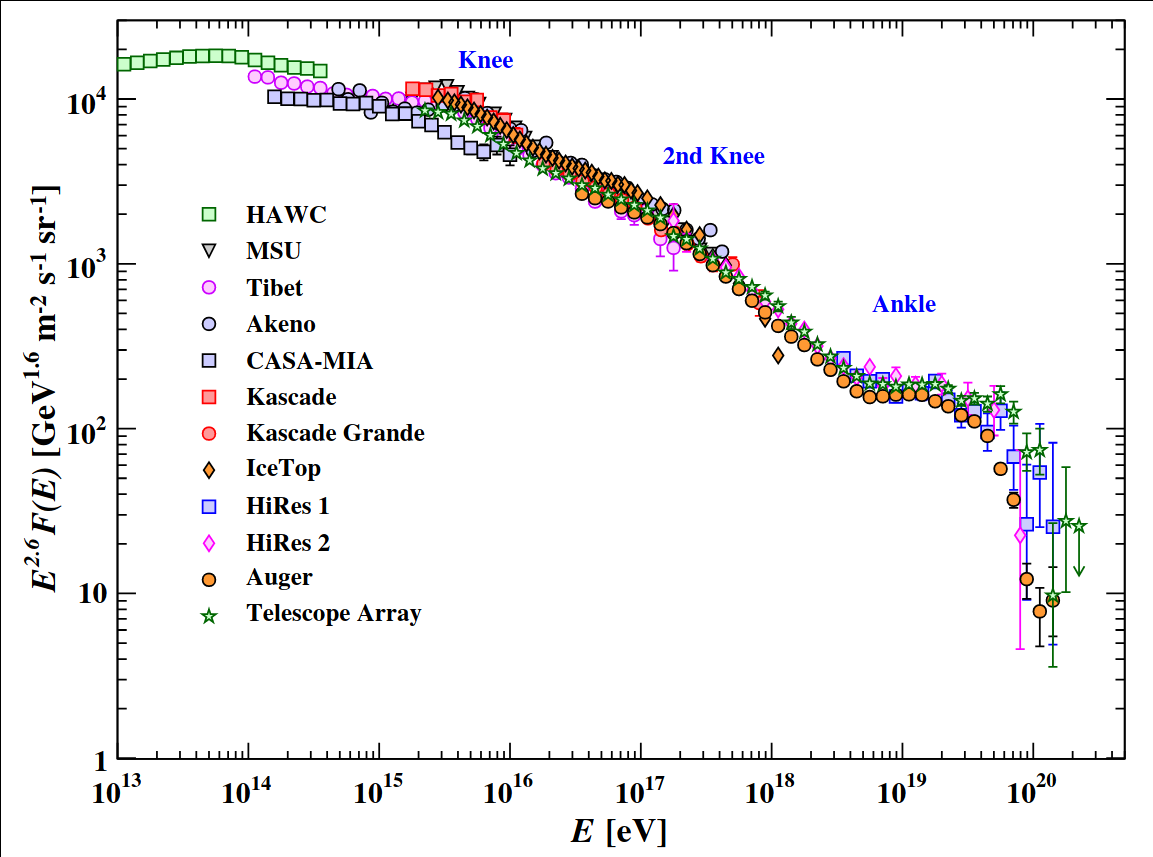
\includegraphics[width=.8\textwidth]{images/cr_spectrum.png}
	\label{fig:multi_messenger}
	\caption{Visualisation of the behaviours of different astronomy messengers. Photons and neutrinos 
		travel the universe without deflection. Charged cosmic rays get deflected by interstellar
		magnetic fields and thus do not allow for a assignment to a cosmological source.
		Neutrinos interact way less than photons both in the universe and in the detector 
		which requires the detectors to be of huge areas. Gravitational waves anyone?
	}
\end{figure}


\subsection{Charged cosmic rays}
The term charged cosmic rays summates all types of charged particles from
extra terrestrial sources with the main proportion seemingly being protons
\cite{something something}


Cosmic rays can similarly be observed both directly and indirectly (werte falsch, anpassen).
- kurze erklärung davon


Figure \ref{fig:cr_spectrum} shows the flux of charged cosmic rays over 
many orders of magnitude in energy which mainly follows 
a power law $E^{-\gamma}$ with gamma somewhere between 
2.7 and 3.3. Deviations from this crude approximation are 
usually referred to as the first and second knee and the ankle 
at $5 10^{15}, 2 10^{17} and 5 10^{18}$ eV respectively.

\begin{figure}
	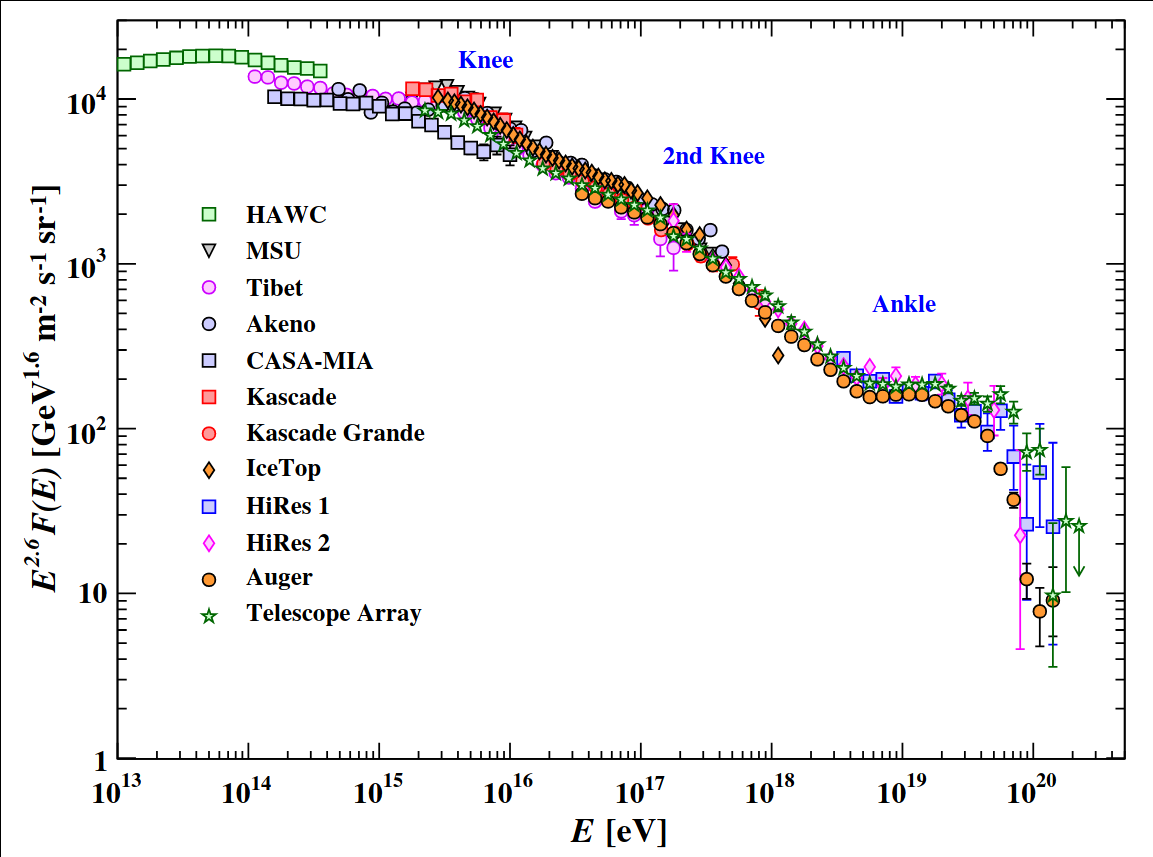
\includegraphics[width=.8\textwidth]{images/cr_spectrum.png}
	\label{fig:cr_spectrum}
	\caption{Combined plot of the cosmic ray spectrum, measured by different air shower experiments. \cite{pdg2019}. 
		The original data were taken from reports from \cite{Alfaro:2017cwx}, 
		\cite{1991ICRC....2...85F}, more here. or leave it altogether.
	}
\end{figure}


At the very highest energies, the flux seems to rapidly decrease, which may point towards a maximum energy
tat cosmological sources can produce or towards destructive interaction with 
the cosmic microwave background \cite{bookap}.

\subsection{Electromagnetic radiation}
In contrast to charged cosmic rays, $\gamma$-particles point towards
their sources, allowing to search for sources of radiation.
In astronomy electromagnetic radiation refers to $\gamma$-particles at all wavelength,
the term $\gamma$-radiation being assigned to the very highest energy particles.
The energy span is usually divided into different ranges, as can be seen in \ref{fig:em_spectrum}

\begin{figure}
	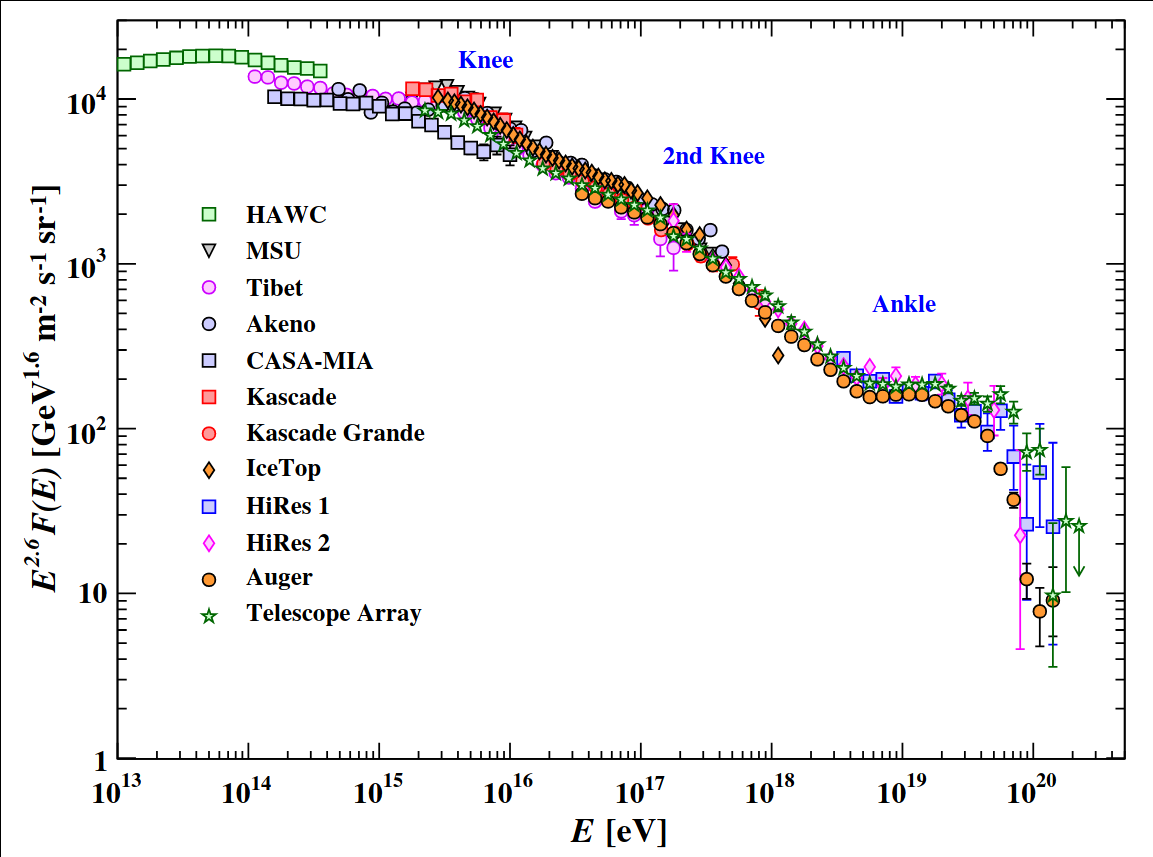
\includegraphics[width=.8\textwidth]{images/cr_spectrum.png}
	\caption{Search for another pic in a paper and cite properly}
	\label{fig:em_spectrum}
\end{figure}


Emitted photons can be observed either directly
from outside the atmosphere via satellites or indirectly
via ground based gamma astronomy. In the later case
IACT's are used to detect electromagnetic showers induced
by the collision of high energy photons with partticles in the atmosphere.
An example for direct observation could be the Fermi satellite (citation needed),
an example for ground based observation could be the
MAGIC-experiment (citation needed).

- smth bout the spectrum with image, bookap has smth but we might find a better one.

\subsection{Neutrinos}
Even less affected by interations on the way from the source to the earth are neutrinos.
Due to their small interaction cross sections and no electric charge, they 
suffer very little from absorption or deflection.
For very much the same reasons detecting neutrinos is much harder
than detecting photons or charged particles.

The small cross section requires to build huge detectors, 
the ICECUBE having a detector volume of \SI{1}{\kilo\meter^3}(cite that).

because of
their small cross-sections. This leads to thousands (größenordnung checken) of
neutrinos passing us continiusly without us even noticing.
For this reason neutrino detectors need to be very large. One example
of such a detector is the ICECUBE detector in ??? (ctation needed).

\subsection{Gravitational waves}
Gravitational waves are the newest channel available for observation.
We can detect them using large size interferometers such as
the LiGO's three detectors (citation needed).



Ground-based cherenkov astronomy focuses on either $\gamma$-rays or cosmic rays


\section{Detection of gamma-rays with ground based telescopes}
The primary particles of gamma or cosmic rays cannot be 
observed with IACTs directly. Instead one can measure the secondary particles
that emerge from the particles interaction with matter.

If the primary energy is high enough, the resulting 
particles can interact with the atmosphere themself, thus starting a 
cascade of secondary particles.

Depending on whether the primary particle is 
a photon/electron/positron or a heavier particle such as a proton 
or iron core, the interactions vary.

This leads to the separation of electromagnetic and hadronic showers.
If the experiment is primarly looking for 
gamma rays, e.g. if measuring a known source like the Crab Nebula, 
the hadronic showers can be treated as background.
As hadronic showers get observed much more frequently, 
the identification of the primary particle type is a very important 
task, often times referred to as gamma-/hadron-separation.

To understand how these showers differ, we will have a very brief look
at the relevant interactions (at primary particle energies in the 
region of modern IACTs).
!!Energiebereiche besser einschränken!!!


\subsection{Electromagnetic showers}
Electromagnetic showers consist mainly of three types of particles:
\begin{enumerate}
	\item{Photons $\gamma$}
	\item{Electrons $e^-$}
	\item{Positrons $e^+$}
\end{enumerate}

The main interaction for high energy photons is pair 
production, generating an $e^+-/e^--$pair where the energy of 
the secondary particles equals the photon energy.
On the other hand high energy electrons (and positrons) lose 
most of their energy by radiation, leading to a photon with 
an energy close to the electron energy.

Only at lower particle energies other interaction forms show their impact,
with particle scattering and ionisation 
leading to more continous energy losses.

Although the energy losses are mainly negligible, 
the most important interaction for the detection with IACTs is 
cherenkov radiation: High energy charged particles pass through 
matter faster than the speed of light in the medium. This leads
to the emittance of near-visible photons that get detected 
in the telescopes camera. 

These assumptions lead to the most basic model of an 
electromagnetic shower, proposed by Bhabha and Heitler in 1937
\cite{doi:10.1098/rspa.1937.0082}.
Today monte carlo calculations get used to simulate the properties 
of particle showers in the atmosphere.
The most common software in the field of IACTs is referred to as
CORSIKA \cite{Engel:2018akg}.


\subsection{Hadronic showers}

\subsection{Measuring events}
% arten von quellen und wie sie beobachtet werden -> welche arten von experimenten beobachten was? wofür sind iacts besonders gut?
